\documentclass[11pt]{scrartcl}
\usepackage{ucs}
\usepackage{float}
\usepackage[utf8x]{inputenc}
\usepackage{ngerman}
\usepackage{amsmath,amssymb,amstext}
\usepackage{graphicx}
\usepackage{tabularx}
\usepackage[square]{natbib}
\usepackage[justification=RaggedRight, singlelinecheck=false]{caption} 
\usepackage{fancyhdr}

\pagestyle{fancy}
\lfoot{Philipp Adler}
\rfoot{\today{}}

\title{Sicherheit}
\author{Philipp Adler}
\date{\today{}}

\begin{document}

\maketitle
\tableofcontents
\pagebreak

\section{Grundlagen Securityverfahren}
\label{sec:basics-security-process}
% Moderne Kryptographie 2

\subsection{Verschlüsselungsarten}
\label{sec:ciphering types}

\subsection{Kommunikationsszenarien}
\label{sec:communication-scenarios}

\subsection{Sicherheitsziele}
\label{sec:security goals}

\subsection{Bedrohungsszenarien}
\label{sec:threat scenarios}


\section{Symmetrische Verschlüsselung}
\label{sec:symetric-ciphering}
Die symmetrische Verschlüsselung reicht bis in die Antike. Damals wussten nur die Adressierten von dem Geheimnis, nach welchem Verfahren die Botschaft verschlüsselt wurde. Cäsar zum Beispiel verschob jeden Buchstaben um 4 Stellen. So wurde aus Hallo Kdoor. Aus diesem Verschlüsselungsalgorithmus entstanden zum einen Blockchiffren, auf den ich in dem folgenden Kapitel näher eingehen werde und die Stromchiffren.\cite{1}

\subsection{Blockchiffre}
\label{sec:blockchiffre}
% Praktische Kryptographie unter Linux 2.3
% Sicherheit und Kryptographie im Internet 1.4.2
Blockchiffren teilen die Nachricht, die verschlüsselt werden soll, in eine fixe Anzahl an Blöcken, die entweder 64 oder 128 Bit groß sind. Typische, bekannte Blockchiffre sind Data Encryption Standard, Advanced Encryption Standard und International Data Encryption Algorithm.\cite{1}
\subsubsection{Der Data Encryption Standard - DES}
\label{sec:data-encryotion-standard}
\grqq{}DES wurde 1977 vom amerikanischen 'National Institute of Standards and Technologies (NIST)' veröffentlicht.\grqq{} \cite{1} Bei diesem Verfahren wird eine Blocklänge von 64 Bit und ein DES-Schlüssel von 56 Bits plus 8 \grqq{}Parity Check Bits\grqq{} \cite{1} eingesetzt. Die ersten 56 Bits werden immer zufällig generiert, wobei die letzten 8 Bits dafür sorgen, dass keine Übertragungsfehler auftreten. Da 56 Bit zufällig sind, können daraus 2\textsuperscript{56} Schlüsseln erzeugt werden. 16 Runden wird ein Block in einen 64 Bit großen Ausgabeblock umgewandelt. Bei jedem Durchgang wird ein anderer Schlüssel für die Verschlüsselung angwendet.
\cite{1}\cite{4}

\noindent \textbf{Das Schema}\\
Beim Verschlüsselungsverfahren wird der Klartext in Blöcke umgewandelt, welche alle jeweils eine Länge von 64 Bit haben, Eingangspermutation IP. Dieser Block wird dann nochmals zerlegt, sodass daraus 2 mal 32 Bit Blöcke entstehen. Der Data Encryption Standard besteht aus 16 Runden. In jeder Runde wird auf die rechte Hälfte ein Verschlüsselungsalgorithmus \textit{f} angewendet.\\
\textit{f} ist in unserem Fall die Rundenfunktion, welche aus 56 zufälligen Bits 48 Bits auswählt. Diese werden mit den 32 Bit der rechten Hälfte, die auf 48 Bit expandiert wurden, mittels XOR-Gatter verknüpft. Die 32 Bit Blöcke werden in 4 aufgeteilt und bekommen zusätzlich am Rand die Nachbarbit. \\
\begin{figure}[H]
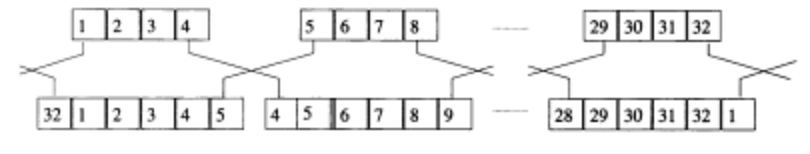
\includegraphics[width=0.60\textwidth]{Bilder/DES/DES_Expansionsabbildung}
	\caption{Expansionsabbildung des DES \citep{2}}
	\label{fig1}
\end{figure}
\noindent \grqq{}Die resultierenden 48 Bits werden in acht Blöcke zu je sechs Bits aufgeteilt\grqq{} \cite{2}, welche als Input für das S-Boxen angewandt werden. Die Substitution-Box besteht aus einer 4 * 16 Matrix, \grqq{}wobei in jeder Zeile eine Permutation der Zahlen von 0,...,15 steht.\grqq{} \citep{2} Die beiden Randbit der Blöcke entscheiden die Zeile und der Rest, die inneren Bit der Blöcke, die Spalte der Substitution-Box. Die ausgewählte Zahl wird dann binär als 4 Bit Block angegeben.\cite{2}
\begin{figure}[H]
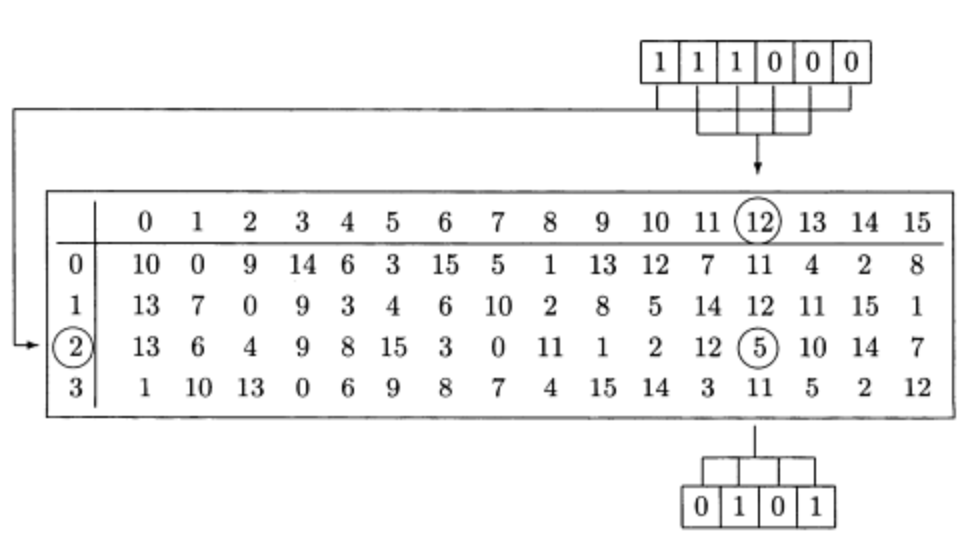
\includegraphics[width=0.45\textwidth]{Bilder/DES/S-Box}
	\caption{S-Box\citep{2}}
	\label{fig2}
\end{figure}
\noindent Da wir nun wieder acht Blöcke zu je 4 Bit haben, können diese zu 32 Bit zusammengefasst werden.\cite{2}
\begin{figure}[H]
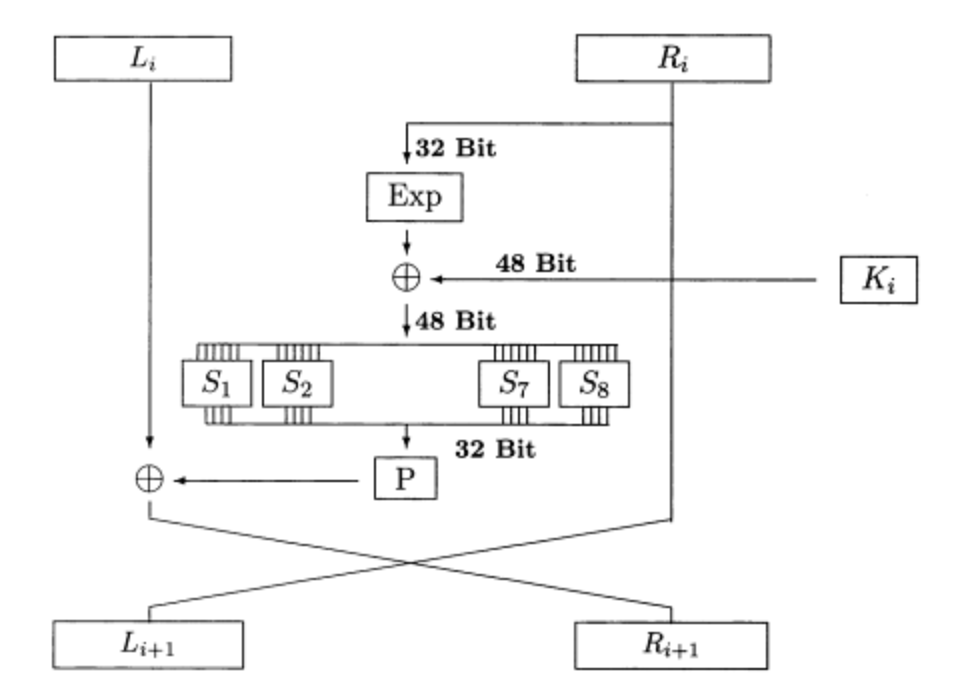
\includegraphics[width=0.45\textwidth]{Bilder/DES/DES_Rundenfunktion}
	\caption{Die DES-Rundenfunktion \citep{2}}
	\label{fig3}
\end{figure}
\noindent Das daraus resultierende Ergebnis wird nochmals permutiert und bitweise mit einem XOR-Gatter mit der linken Hälfte verknüpft und \grqq{}bildet die rechte Seite der neuen Runde.\grqq{} Unter permutiert versteht man, dass jedes einzelne bit als Zahl dargestellt wird und mit 8 addiert wird.\cite{2}
\begin{figure}[H]
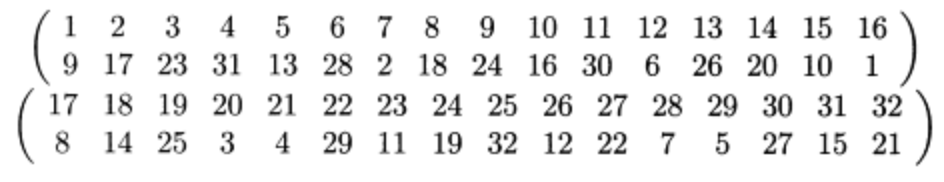
\includegraphics[width=0.40\textwidth]{Bilder/DES/DES_Permutation}
	\caption{Permutation de DES \citep{2}}
	\label{fig4}
\end{figure}
\noindent 
Da der 48 Bit Schlüssel, welcher vom 56 Bit-Hauptschlüssel hergeleitet wird, bei jeder Runde ein anderer ist, muss dieser irgendwie generiert werden. Der Hauptschlüssel wird permutiert und die Funktion PC-1 teilt diesen in 2 Blöcke zu je 28 Bit. Bei der Permutierung werden die 8 Paritätsbit entfernt, die Bits mit der Nummer 8, 16, 24, 32, 40, 48, 56, 64, wobei nur noch 56 Bit übrig bleiben. Jede der beiden Hälften wird bei jeder Iteration zirkulärisch links für die Verschlüsselung, nach rechts für die Entschlüsselung gesshiftet. Das heißt, dass jeder Block entweder ein oder zwei Bit nach links rotiert und auf 24 Bit extrahiert wird. So kann es nicht vorkommen, dass ein Rundenschlüssel nicht zweimal angewendet wird.\\
\grqq{}Nach 16 Runden werden die 64 Bit einer Ausgangspermutation unterzogen\grqq{} \cite{2}, woraus der Geheimtext resultiert. Die Ausgangspermutation ist die inverse von der Eingangspermutation, dass heißt alle 64 Bit Blöcke werden zu einem Geheimtext zusammengeführt. Nachteil dieser Implementierung ist, dass die Ein- und Ausgangspermutation öffentlich sind und so von Angreifern berechnet werden können, was die Sicherheit drastisch verringert.
\cite{2}\cite{4}
\begin{figure}[H]
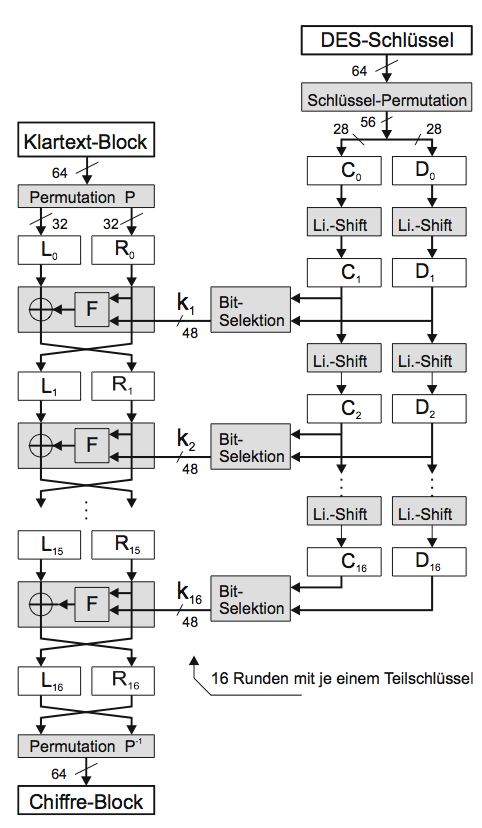
\includegraphics[width=0.40\textwidth]{Bilder/DES/DES_Schema}
	\caption{DES-Verschlüsselung-Schema \citep{3}}
	\label{fig5}
\end{figure}
% Kryptografie in Theorie und Praxis 7.6
% Kryptograhie und IT-Sicherheit 2.2
% Verteilte Systeme S.427

\subsubsection{Der Advanced Encryption Standard - AES}
\label{sec:advanced-encryotion-standard}
Da der DES-Algorithmus aus einen verhältnismäßig kurzen 56-Bit Schlüssel besteht und dieser 1999 durch einen sogenannten Brute-Force-Angriff in 22 Stunden geknackt wurde, müssen andere Vorschläge her. Die Alternative hieß AES, Advanced Encryption Standard, ist ebenfalls eine symmetrische Block-Chiffre, mit einer Blocklänge von 128 Bit.
\cite{3}

\noindent \textbf{Das Schema}\\
Der Unterschied zum DES ist, dass AES eine flexible Block- und Schlüssellänge besitzt. Der Standard besitzt eine standardisierte Blocklänge von 128 Bit und Schlüssellängen von 128 Bit, 192 Bit und 256 Bit. Wieviele Runden absolviert werden hängt von der Schlüssellänge ab. 10 Runden bei einer Schlüssellänge von 128 Bit, was derzeit der Standard ist, 12 Runden bei 192 Bit und 14 Runden bei 256 Bit. \grqq{}Vor der ersten Runde wird ein Rundenschlüssel mit dem Klartext XOR-verknüpft.\grqq{}\citep{2}
\cite{3}
\begin{figure}[H]
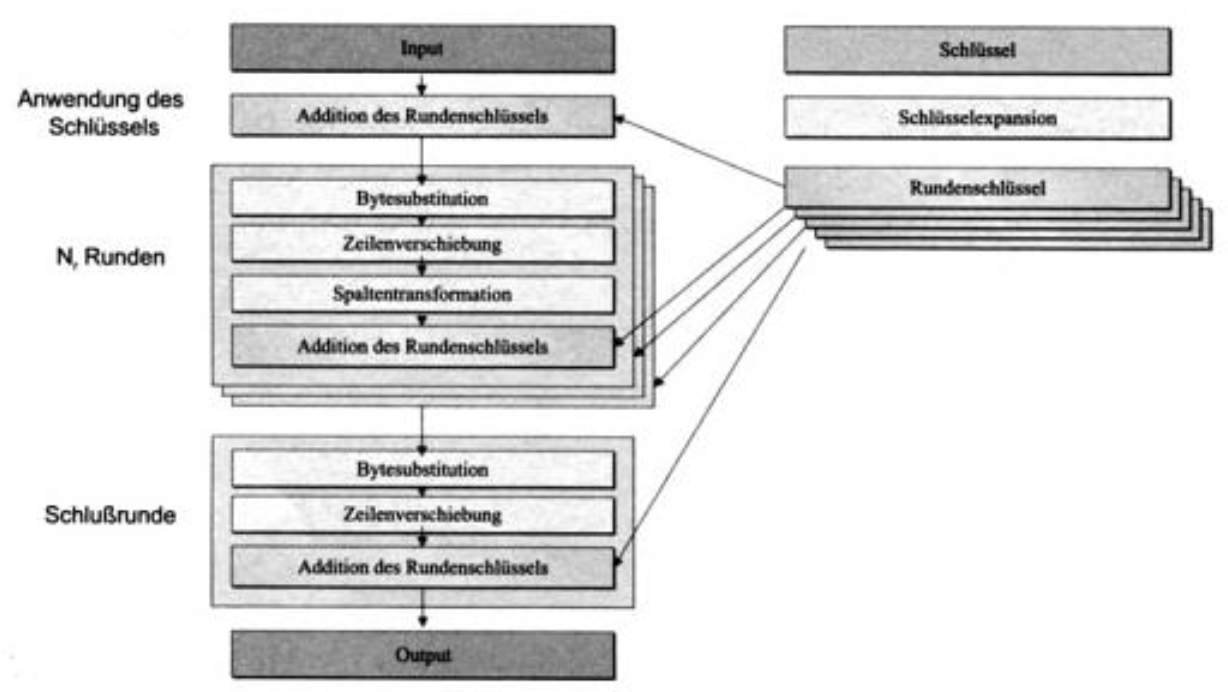
\includegraphics[width=0.40\textwidth]{Bilder/AES/AES_Schema}
	\caption{Schema des AES \citep{2}}
	\label{fig6}
\end{figure}
\noindent 
Beim AES wird der Text und die Ergebnisse als Bytes in eine 4x4-Matrix, in sogenannte States, gespeichert. Die Einträge erfolgen spaltenweise, wobei von links nach rechts angeordnet wird. Bei dieser Transformationsfunktion werden die 128 Bit in 16 Bytes geteilt. Diese Bytes werden als States in der Matrix bezeichnet. Die Suche erfolgt mittels der Indexe.
\cite{2}\cite{3}
\begin{figure}[H]
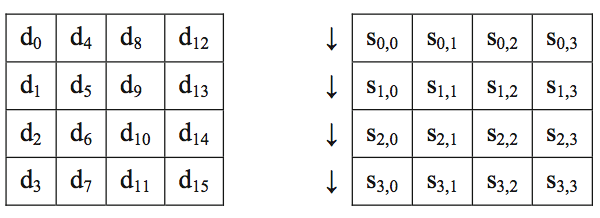
\includegraphics[width=0.40\textwidth]{Bilder/AES/AES_State}
	\caption{Datenstruktur: ein State \citep{3}}
	\label{fig7}
\end{figure}
\noindent
Wie auch DES eine Rundenfunktion besitzt, hat AES ebenfalls eine. Diese besteht aus SubBytes, ShiftRow, MixColumn und AddRoundKey.\\
Beim SubBytes werden die States substituiert. Zuerst wird das Eingangsbyte durch die gebildete Inverse a{\tiny r,c} ersetzt.
\grqq{}Entscheidend für das Verständnis des AES ist, dass die Bytes als Elemente des Körpers \textit{GF}(2\textsuperscript{8}) aufgefasst werden.\grqq{}\citep{2} Dadurch ist es möglich Bytes zu addieren und multiplizieren. Dieser Körper wird durch Polynome in Form als \textit{GF}(2)[\textit{x}]/(\textit{x}\textsuperscript{8} + \textit{x}\textsuperscript{4} + \textit{x}\textsuperscript{3} + \textit{x} + \textit{1}) dargestellt. Für die Berechnung wird das Byte in Bits dargestellt und einem Polynom zugeordnet. Es wird dann nicht mehr mit Bytes gerechnet sondern mit Polynomen.\\
\textit{{10100010} = x\textsuperscript{8} + x\textsuperscript{6} + x}
Der neue State wird mit einer 8x8 Matrix mod 2 multipliziert. Daraus ergibt sich ein Byte großer Ergebnisvektor der zum Schluss mit der Konstante GF(2\textsuperscript{8}) addiert wird. Vorteil an diesem Algorithmus ist das die Bildung der Inverse eines Bytes nichtlinear ist, was die Analyse des AES erschwert.\cite{2}\cite{3}\\
\begin{figure}[H]
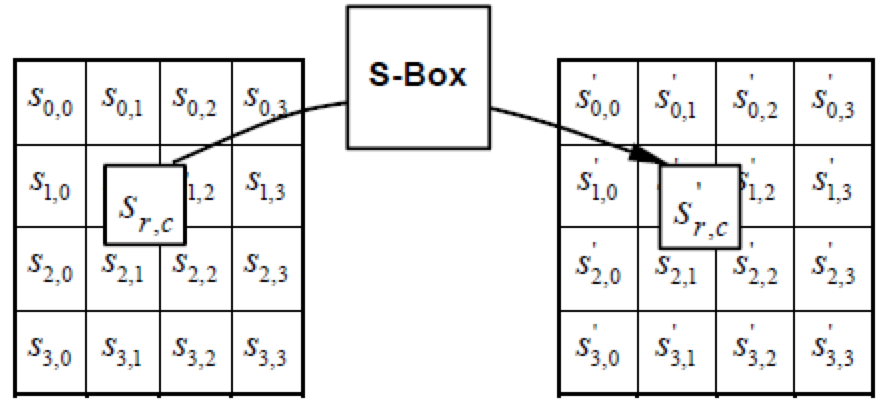
\includegraphics[width=0.40\textwidth]{Bilder/AES/AES_SubBytes}
	\caption{Die Abbildung SubBytes \citep{2}}
	\label{fig8}
\end{figure}
\noindent
ShiftRow und MixColumn stellen die Permutation der Rundenfunktion dar. Wobei ShiftRow zeilenweise operiert und MixColumn spaltenweise. Beim ShiftRow besteht die Permutation aus einem Linksshift, welcher von der Blocklänge abhängig ist. Ausgenommen ist die erste Zeile, weil diese nie verschoben wird. Ansonsten wird die 2.Zeile um C1 Bytes, die 3.Zeile um C2 und die 4.Zeile um C3 Bytes verschoben. Falls die Blocklänge 128 Bit beträgt, wird wie folgt nach Links geshiftet.\cite{2}
\begin{figure}[H]
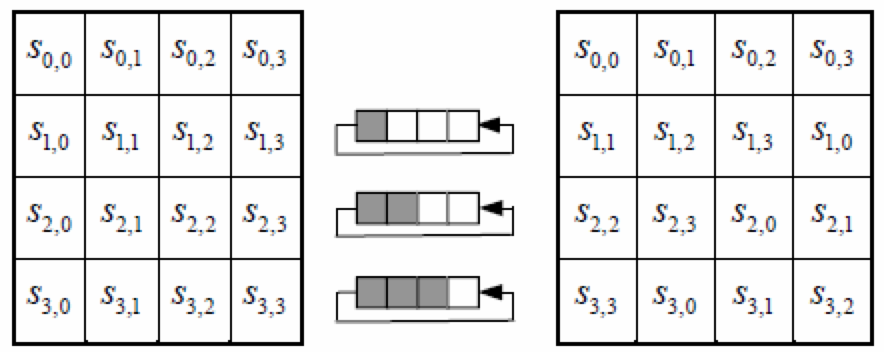
\includegraphics[width=0.40\textwidth]{Bilder/AES/AES_ShiftRow}
	\caption{Die Abbildung ShiftRow \citep{2}}
	\label{fig9}
\end{figure}
\noindent
Wie schon oben erwähnt kümmert sich der MixColumn um die Spalten, welche aus 4 Byte bestehen, die wie bei SubBytes als Polynom dargestellt werden. Da wir hier nur 4 Byte haben, ist der Grad kleiner gleich 3. Das daraus erzeugte Polynom wird mit einer Konstante mod (x\textsuperscript{4} + 1) multipliziert.\cite{2}
\begin{figure}[H]
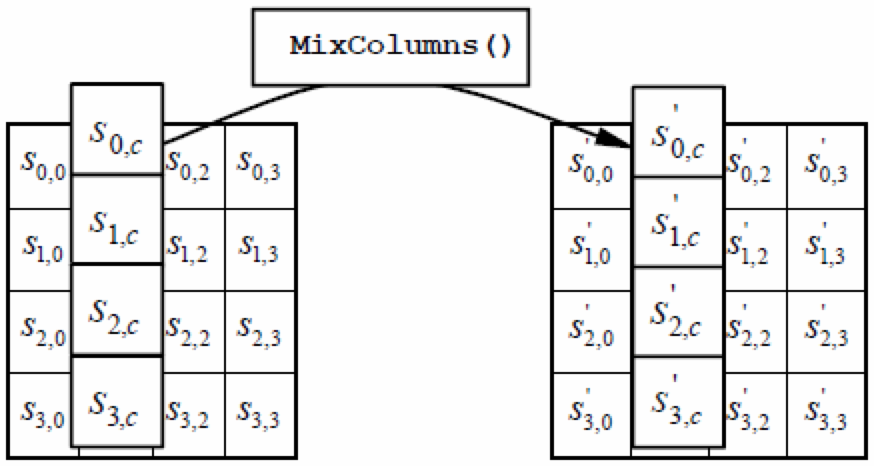
\includegraphics[width=0.40\textwidth]{Bilder/AES/AES_MixColumn}
	\caption{Die Abbildung MixColumn \citep{2}}
	\label{fig10}
\end{figure}
\noindent
AddRoundKey wird vor Beginn der Runden und am Ende jeder Runde eingesetzt. Um den aktuelle Rundenschlüssel und der Block mittels einer XOR-Verknüpfung addiert. Der Rundenschlüssel wird durch die Formel (Rundenanzahl + 1) * (Anzahl der Wörter pro Matrix) hergeleitet. Da bei 128 Bit mehr Bits zur Verfügung stehen als benötigt werden, muss der Schlüssel expandiert werden. Bei der Expansion wird der externe Schlüssel in seine Bestandteile zerlegt, was im Falle von 128 Bit 4 Wörter sind. Dabei wird i und i+3 mittels XOR verknüpft.\\
In jeder neuen Runde werden andere Rundenschlüssel verwendet, indem man in der Ersten die ersten vier Wörter und in den nächsten die nächsten vier verwendet.\citep{2}

% Kryptografie in Theorie und Praxis 7.7
% Kryptograhie und IT-Sicherheit 2.6

% Moderne Kryptographie 4.5

\subsubsection{IDEA (International Data Encryption Algorithm)}
\label{sec:international-data-encryption-algorithm}
Der International Data Encryption Algorithm ist ebenfalls wie DES und AES eine symmetrische Block-Chiffre, welche aus einer Blocklänge von jeweils 64 Bit und einer Schlüssellänge von 128 Bit besteht.\citep{3}

\noindent \textbf{Das Schema}\\
Das IDEA besteht aus 9 Runden, wobei die ersten 8 Runden alle den gleichen Vorgang ausführen. Der Klartext bestehend aus 64 Bit wird in 4 Blöcke aufgespalten. Der erste und letzte Block wird mit einem Teilschlüssel modulo (2\textsuperscript{16} + 1) multipliziert, weil da immer ein Rest auftretet, da es sich um eine Primzahl handelt. Die inneren Blöcke werden stattdessen modulo (2\textsuperscript{16}) addiert. In der Mitte des Schemas werden 2 andere Teilschlüssel eingesetzt, welche die Ergbnisse von oben addieren oder multiplizieren. Am Ende jeder Runde werden die innen Ausgänge vertauscht. Da in jeder Runde ein anderer Klartext zum Einsatz kommt, werden auch andere Teilschlüssel angewandt. \grqq{} Aus den Primärschlüssel werden 52 Teilschlüssel von 16 Bit Länge erzeugt, von denen je sechs in acht Runden zum Einsatz kommen.\grqq{}\citep{6}
Da die ersten 8 Runden nun beschrieben wurden, kommen wir zur letzten. Bei der 9ten Runden wird der Hauptteil des Verschlüsselungsschemas ausgelassen, dagegen werden 4 Teilschlüssel k{\scriptsize 9,1}, k{\scriptsize 9,2}, k{\scriptsize 9,3}, k{\scriptsize 9,4} eingesetzt.\citep{3}\citep{6}
\begin{figure}[H]
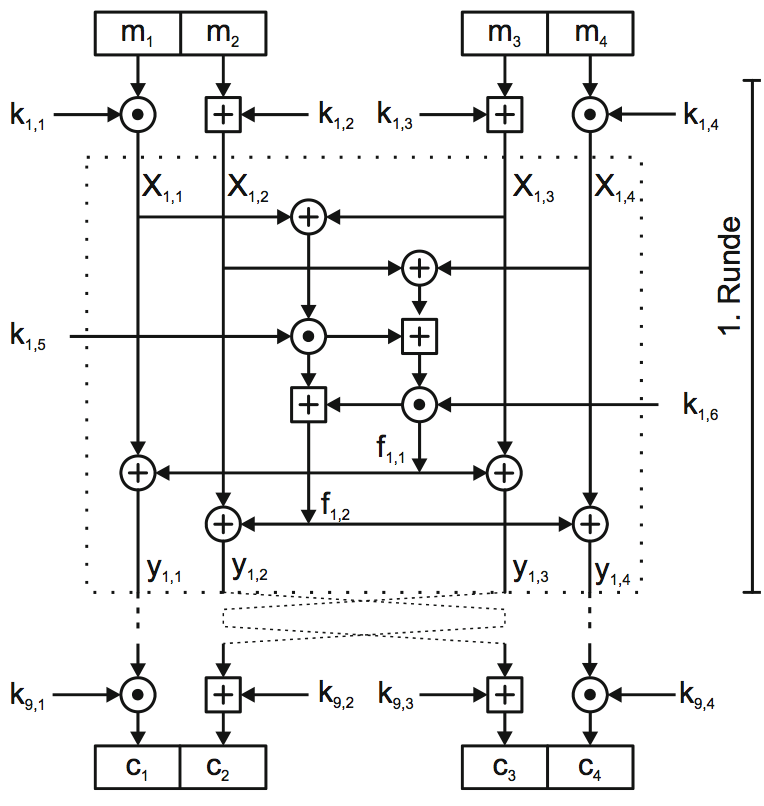
\includegraphics[width=0.40\textwidth]{Bilder/IDEA/IDEA_Schema}
	\caption{IDEA Schema \citep{3}}
	\label{fig11}
\end{figure}
\noindent
Die Entschlüsselung funktioniert wird die Verschlüsselung nur in andere Richtung, nur die Teilschlüssel k{\scriptsize 9,x} werden invertiert. \citep{3}
% Kryptograhie und IT-Sicherheit 2.3

\subsection{Der RSA-Algorithmus}
\label{sec:rsa-algorithmus}
Eines der bekanntesten Public-Key-Verfahren ist der RSA-Algorithmus. Entwickelt wurde es 1977 von Rivest, Shamir, Aleman. Das Verfahren beruht auf der Schwierigkeit der Faktorisierung von Zahlen, der sogenannte Satz von Euler. Beim RSA wird ein Nachrichtenblock als Zahl interpretiert, welche kleiner als modula \textit{n} ist. \citep{2}
% 6.Praktische Kryptographie unter Linux 2.4.3
% 2.Kryptografie in Theorie und Praxis 10
% 3.Kryptograhie und IT-Sicherheit 4.2
% 5.Moderne Kryptographie 6.4
% 1.Sicherheit und Kryptographie im Internet 1.5.4

\subsubsection{Schlüsselerzeugung}
\label{sec:key-generation}
Für die Erzeugung des Schlüssels \textit{n} benötigt man das Produkt von zwei Primzahlen \textit{p} und \textit{q}, die mindestens 512 Bit lang sind 2\textsuperscript{512} und geheim gehalten werden. Die Wahrscheinlichkeit, dass es sich um eine Primzahl handelt ist 2\textsuperscript{-9}. Um das faktorisieren zu erschweren gibt spezielle Kriterien. Erstens die Primzahlen sollten sich nicht sehr unterscheiden, aber nicht beieinander liegen. Für die Teilfremdezahl sollte man möglichst kleine Teiler haben.\\
Als nächstes wird eine Zahl \textit{e}, enciphering, die teilfremd zu $\varphi(n)$ = (p - 1)(q - 1) ist, ausgewählt. Unter Teilfremd versteht man, dass die beiden Zahlen keinen gemeinsamen Teiler haben. Mit diesen beiden Zahlen kann der öffentliche Schlüssel (\textit{e, n}) gebildet werden. Damit der Empfänger die Nachricht entschlüsseln kann, benötigt er einen privaten Schlüssel \textit{d}. Die Zahl \textit{d} wird mit Hilfe des Euklidischen Algorithmus \textit{e * d mod (p - 1)(q - 1) = 1} berechnet.\\
\textbf{RSA-Signatur}\\
\grqq{}Mit Hilfe des RSA-Verfahrens kann man auch leicht eine digitale Signatur realisieren: Man bildet zunächst den Hashwert \textit{h = hash(m)} der zu signierenden Nachricht \textit{m}, und berechnet die Signatur, indem man diesen Hashwert 'entschlüsselt'.\grqq{}\citep{1}
Um die Signatur zu prüfen, wird der Hash des Dokuments nochmal gebildet und \grqq{} dann der Wert \textit{sig} durch Potenzierung mit dem öffentlichen Schlüssel \textit{e} 'entschlüsselt' wird.\grqq{}\citep{1}.
Wenn beide übereinstimmen war die Signatur korrekt.
\citep{1}\citep{2}\citep{6}
\subsubsection{Verschlüsseln}
\label{sec:rsa-encrypt}
Bei der Verschlüsselung wendet der Sender den öffentlichen Schlüssel des Empfängers an seinen Nachrichtenblock an.\\
\textit{c} = \textit{m}\textsuperscript{e} (mod \textit{n})\\


\subsubsection{Entschlüsseln}
\label{sec:rsa-decrypt}
Der Empfänger muss nur noch seinen privaten Schlüssel auf den Geheimtext \textit{c} zum Entschlüsseln anwenden.\\
\textit{m} = \textit{c}\textsuperscript{d} (mod \textit{n})\\

\section{SSL/TLS-Protokoll}
\label{sec:ssl/tls-protocol}
% Praktische Kryptographie unter Linux 8.1
% Kryptograhie und IT-Sicherheit 6.3
% Sicherheit und Kryptographie im Internet 7.7/7.9
% Verteilte Systeme S.626

\subsection{SSL/TLS Grundlagen}
\label{sec:ssl-tls-basics}

\subsection{SSL/TLS im Protokollstapel}
\label{sec:ssl-tls-protocolstack}

\subsection{Client-Server-Kommunikation}
\label{sec:client-server-communication}



\subsection{Das SSL-Handshake}
\label{sec:ssl-handshake}

\subsection{TLS asymetrisch}
\label{sec:tls-asymetric}

\subsection{TLS symetrisch}
\label{sec:tls-symetric}

\subsection{TLS hybrid}
\label{sec:tls-hybrid}

\subsection{TLS Algorithmen}
\label{sec:tls-algorithmen}


\section{Schwierigkeiten bei Software}
\label{sec:sw-trouble}

\subsection{Buffer Ovrflow}
\label{sec:buffer-overflow}
% Improving Intrusion Detection Systems 4.3
% Network Intrusion Detection and Prevention 1.3.1

\subsection{OpenSSL}
\label{sec:openssl}
% Praktische Kryptographie unter Linux 8.2
% Sicherheit und Kryptographie im Internet 7.10

\newpage
\listoffigures
\addcontentsline{toc}{section}{Abbildungsverzeichnis}
\addcontentsline{toc}{section}{Literaturverzeichnis}
\mbox{}
\nocite{*}
\bibliographystyle{unsrt}
\bibliography{literatur}

\end{document}